\documentclass[12pt,letterpaper]{article}

% Only use basic packages that are always available
\usepackage[utf8]{inputenc}
\usepackage[T1]{fontenc}
\usepackage[margin=1in]{geometry}
\usepackage{amsmath}
\usepackage{amsfonts}
\usepackage{amssymb}
\usepackage{graphicx}
\usepackage{url}
\usepackage{float}


% Title page information
\title{
    \vspace{2in}
    \textbf{\Automated RAG Chatbot Development using Cursor IDE:\\
    A Comprehensive Framework for Secure Data Querying} \\
    \vspace{0.5in}
    \large MSDS 7335 - Machine Learning II \\
    Final Project Report \\
    \vspace{0.5in}
}

\author{
    Tue Vu \\
    Southern Methodist University \\
    Lyle School of Engineering \\
    Master of Science in Data Science \\
    \vspace{0.25in}
}

\date{\today}

\begin{document}

% Title page
\maketitle
\newpage

\textbf{Abstract}

This report presents the development of an automated Retrieval-Augmented Generation (RAG) chatbot system using Cursor IDE AI-powered development environment. The primary objective was to create a secure, locally-deployable chatbot capable of querying sensitive data without relying on external APIs. The system integrates Ollama for local language model inference, Langchain for RAG framework implementation, ChromaDB for vector storage, and Gradio for user interface development. The entire development workflow was automated using Cursor IDE, demonstrating the potential of AI-assisted programming in creating complex machine learning applications. The resulting system provides multiple deployment options including High-Performance Computing (HPC) clusters via Open OnDemand, Kubernetes and cloud deployment through AWS services.
This work contributes to the growing field of secure, privacy-preserving AI applications while showcasing the transformative impact of AI-powered development tools in academic and professional machine learning projects.

Keywords: Retrieval-Augmented Generation, Cursor IDE, Ollama, Langchain, ChromaDB, open-source LLM, AI-Assisted Development

\newpage

\section{Introduction}

In the rapidly evolving landscape of artificial intelligence and machine learning, the need for secure, privacy-preserving solutions for sensitive data analysis has become paramount. Traditional cloud-based AI services, while powerful, often require transmitting sensitive data to external servers, raising significant privacy and security concerns for organizations handling confidential information. This challenge is particularly acute in sectors such as healthcare, finance, and government, where data privacy regulations and security requirements mandate strict control over data access and processing.

The emergence of Retrieval-Augmented Generation (RAG) systems has provided a promising solution for creating intelligent question-answering systems that can work with domain-specific documents while maintaining data privacy. However, developing such systems traditionally requires extensive expertise in multiple technologies, significant development time, and careful integration of various components including language models, vector databases, and user interfaces.

The introduction of AI-powered development environments, particularly Cursor IDE, has revolutionized the software development process by providing intelligent code completion, automated bug fixing, and comprehensive project scaffolding capabilities. 
Cursor represents a paradigm shift in how complex machine learning applications can be developed, enabling researchers and practitioners to focus on high-level design and requirements while the AI assistant handles much of the implementation details.

The primary objective of this project is to demonstrate the feasibility and effectiveness of using Cursor to automatically create a comprehensive RAG chatbot system with the following key requirements:

\begin{itemize}
    \item Local Deployment: No reliance on external APIs call, ensuring complete data privacy and security
    \item Multi-format Support: Capability to process and query PDF and text documents
    \item Flexible Model Selection: Support for multiple local language models with real-time switching
    \item User-friendly Interface: Intuitive graphical interface for non-technical users
    \item Scalable Deployment: Multiple deployment options from personal computers to cloud infrastructure
    \item Automated Development: Minimal manual coding through AI-assisted development
\end{itemize}

This work makes several important contributions to the field:

\begin{itemize}
    \item Demonstrates the practical application of AI-assisted development tools in creating complex ML systems
    \item Provides a comprehensive framework for secure, local RAG implementation
    \item Establishes deployment strategies for various computing environments
    \item Validates the effectiveness of Cursor in academic machine learning projects
    \item Creates a reusable template for similar privacy-preserving AI applications
\end{itemize}

This report is organized into four main chapters. 
Chapter 1 introduces the project and provides a brief overview of the RAG chatbot system. 
Chapter 2 provides detailed technical background on the models and technologies employed, including Ollama, Langchain, ChromaDB, and Gradio, along with a comprehensive explanation of the RAG workflow. 
Chapter 3 describes the automated development process using Cursor and presents various deployment strategies. 
Chapter 4 discusses the results, implications, and conclusions, with particular emphasis on the role and necessity of AI-assisted development tools in modern machine learning workflows.

\newpage

\section{Models and Data}

The RAG chatbot system developed in this project represents a sophisticated integration of multiple state-of-the-art technologies, each serving a specific role in the overall architecture. The system follows a modular design pattern that ensures scalability, maintainability, and flexibility in deployment scenarios.

\begin{figure}[H]
    \centering
    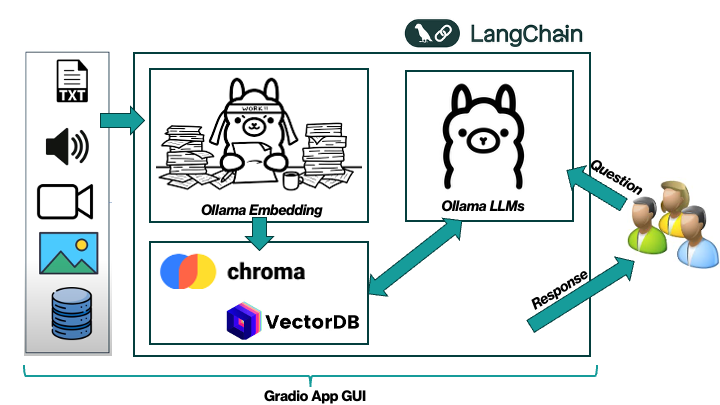
\includegraphics[width=1\textwidth]{plots/Fig1.png}
    \caption{Overall RAG Workflow with its components}
    \label{fig:overall_workflow}
\end{figure}

Figure \ref{fig:overall_workflow} shows the overall RAG workflow with its components. The RAG workflow can take any input in different formats (text, image, audio, video, database).
It then embeds the input into a vector space using the embedding models and store the vectorized input in the database suchas ChromaDB or VectorDB.
Users then can query the database using the query engine to retrieve the most relevant documents.
The retrieved documents are then passed to the language model to generate the response. The entire workflow interface is built using Gradio app.

\subsection{Ollama: Local Language Model Infrastructure}
\label{sec:ollama}

Ollama (ollama.com) serves as the backbone of our local language model infrastructure, providing a robust platform for running large language models on consumer hardware without requiring external API access. This choice was motivated by the project's emphasis on data privacy and the need for a solution that could operate entirely within secured network environments.

The system supports multiple large language models, each optimized for different use cases and computational constraints:

\begin{itemize}
    \item \textbf{Gemma3}: an open‑weights LLM family built on the same technology as Google’s Gemini models, designed to be efficient enough to run on consumer hardware like laptops or GPUs. The latest version Gemma3 has different sizes from 1B, 4B, 12B to 27B parameters and support vision models.
    \item \textbf{DeepSeek-R1}: Optimized for reasoning tasks and complex query processing, having different versions from 1.5B to 671B
    \item \textbf{Llama3}: Meta's latest compact model with improved instruction following, also released in different versions from from 8B to 70B parameters.
    \item \textbf{Qwen3}: Alibaba's multilingual model with enhanced language understanding, offering a comprehensive suite of dense and mixture-of-experts (MoE) models.
    \item \textbf{mxbai-embed-large}: Specialized embedding model from mixedbread.ai for vector representation generation
\end{itemize}

The selection of these models represents a careful balance between performance and resource requirements. The following table provides a detailed comparison of the computational requirements and performance characteristics of each model:

\begin{table}[H]
    \centering
    \caption{Selected LLMs and their performance characteristics in this project}
    \resizebox{\textwidth}{!}{
    \begin{tabular}{|l|c|c|c|l|}
        \hline
        \textbf{Model} & \textbf{Parameters (B)} & \textbf{Memory (GB)} & \textbf{Context Window} & \textbf{Use Case} \\
        \hline
        Gemma3 & 1, 4, 12, 27 & 0.8, 3.3, 8.1, 17.0 & 32k for 1B, 128k for rest & General purpose: Text, Image \\
        \hline
        DeepSeek-R1 & 1.5, 7, 8, 14, 32, 70, 671 & 1.1, 4.7, 5.2, 9, 20, 43, 404 & 128K for all, except 671B: 160k & Reasoning tasks: Text \\
        \hline
        Llama3 & 8, 70 & 4.7, 40 & 8k for all & Instruction following: Text \\
        \hline
        Qwen3 & 0.6, 1.7, 4, 8, 14, 30, 32, 235 & 0.5, 1.4, 2.6, 5.2, 9.3, 19, 20, 142 & 40k for all except 30B and 235B have 256k & Multilingual: Text \\
        \hline
        mxbai-embed-large & 0.3 & 0.7 & 512 & Embeddings \\
        \hline
    \end{tabular}
    }
\end{table}

\subsection{Langchain: RAG Framework Implementation}

Langchain provides the foundational framework for implementing the RAG pipeline, offering a comprehensive set of tools for document processing, vector store integration, and query orchestration. The framework's modular architecture allows for easy customization and extension of the RAG workflow.

The document processing pipeline implemented using Langchain consists of several key stages:

\begin{enumerate}
    \item \textbf{Document Ingestion}: Support for multiple file formats including PDF and plain text
    \item \textbf{Text Extraction}: Robust extraction algorithms handling various document layouts
    \item \textbf{Text Chunking}: Recursive character-based splitting with configurable parameters
    \item \textbf{Metadata Preservation}: Maintenance of source information and document structure
\end{enumerate}

The text chunking strategy employs a recursive approach with the following parameters:
\begin{itemize}
    \item Chunk size: 1000 characters
    \item Overlap: 200 characters
    \item Separators: Paragraph breaks, sentence boundaries, and whitespace
\end{itemize}

\subsection{ChromaDB: Vector Database Management}

ChromaDB serves as the vector database backend, providing efficient storage and retrieval of document embeddings. The choice of ChromaDB was motivated by its simplicity, performance, and compatibility with local deployment scenarios.

The embedding strategy employs the mxbai-embed-large model to generate high-dimensional vector representations of document chunks. This model was selected for its superior performance on semantic similarity tasks and its relatively modest computational requirements.

The retrieval mechanism implements a similarity search using cosine distance metrics, with configurable parameters for result ranking and filtering:

\begin{itemize}
    \item Search depth: Top-4 most similar chunks
    \item Similarity threshold: Dynamically adjusted based on query complexity
    \item Result diversification: Implemented to avoid redundant content
\end{itemize}

\subsection{Gradio: User Interface Development}

The Gradio-based user interface was designed with simplicity and functionality in mind, providing an intuitive experience for users regardless of their technical background. The interface incorporates modern web design principles while maintaining accessibility standards.

The interface consists of several key components:

\begin{enumerate}
    \item \textbf{File Upload Module}: Drag-and-drop interface supporting multiple file formats
    \item \textbf{Model Selection Panel}: Dynamic dropdown for real-time model switching
    \item \textbf{Parameter Controls}: Temperature slider and other model parameters
    \item \textbf{Chat Interface}: Conversational interface with history management
    \item \textbf{Status Indicators}: Real-time feedback on system operations
\end{enumerate}

\subsection{RAG Workflow Implementation}

The complete RAG workflow follows a carefully orchestrated sequence of operations designed to maximize both performance and user experience.

\begin{figure}[H]
    \centering
    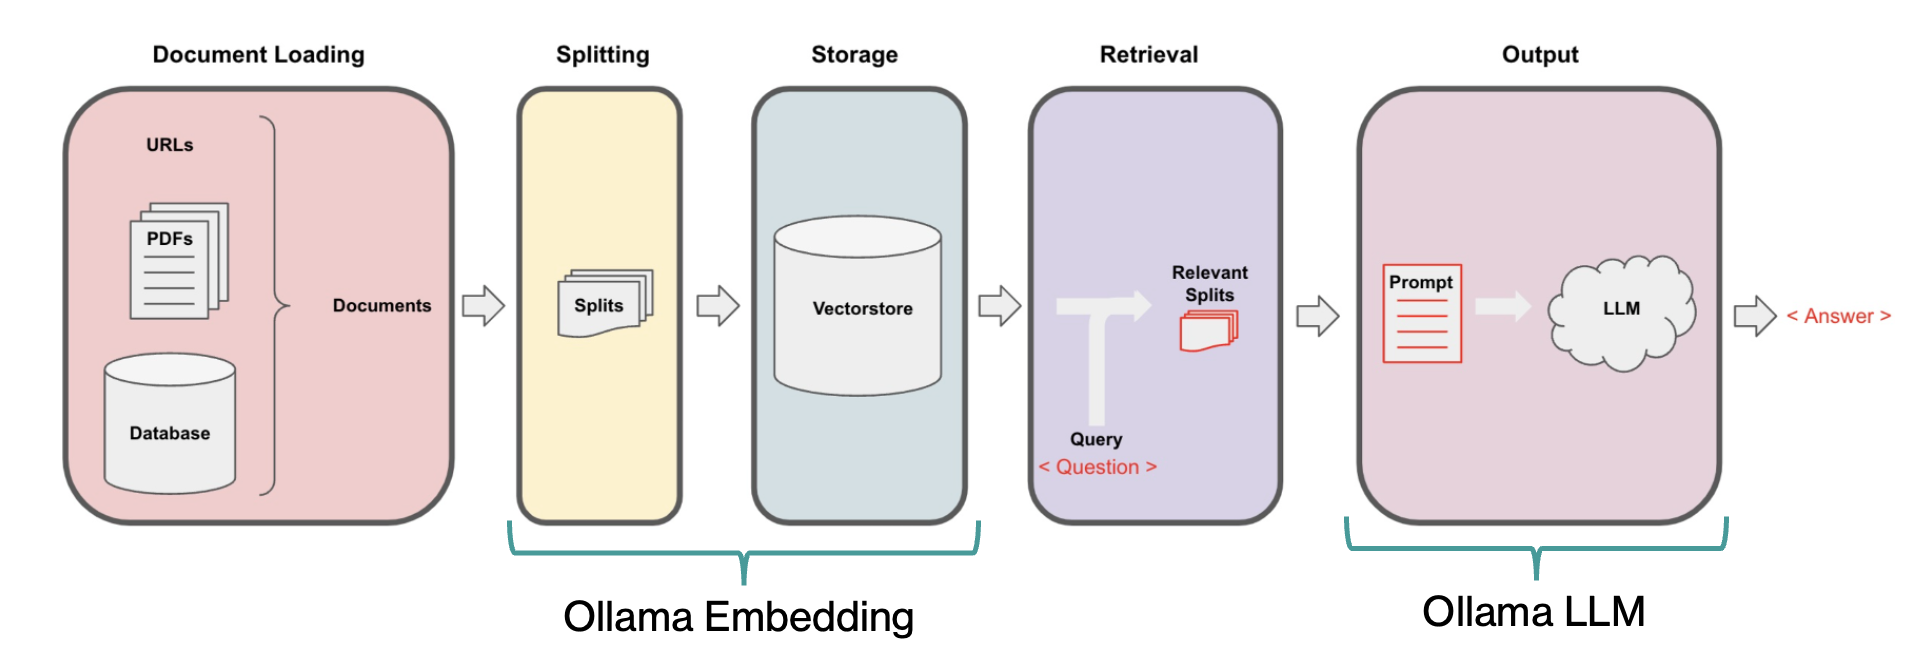
\includegraphics[width=1\textwidth]{plots/Langchain.png}
    \caption{RAG workflow implemented using Langchain}
    \label{fig:rag_workflow}
\end{figure}


The data processing pipeline implements a robust error handling and recovery mechanism to ensure system reliability:

\begin{enumerate}
    \item \textbf{Document Validation}: File format verification and integrity checking
    \item \textbf{Text Extraction}: Fault-tolerant extraction with fallback mechanisms
    \item \textbf{Quality Assessment}: Content quality evaluation and filtering
    \item \textbf{Embedding Generation}: Batch processing with error recovery
    \item \textbf{Storage Management}: Automatic cleanup and optimization
\end{enumerate}

\newpage

\section{Automated Workflow via Cursor IDE}

The development of complex machine learning applications traditionally requires extensive expertise across multiple domains, significant development time, and careful coordination of various technological components. The emergence of AI-powered development environments, particularly Cursor.com, has fundamentally transformed this paradigm by enabling automated code generation, intelligent debugging, and comprehensive project scaffolding.

\subsection{Cursor Development Environment}

Cursor represents a revolutionary approach to software development, combining the power of large language models with traditional integrated development environment (IDE) features. The platform provides several key capabilities that proved instrumental in this project:

\begin{itemize}
    \item \textbf{Intelligent Code Generation}: Context-aware code completion and generation based on natural language descriptions
    \item \textbf{Automated Debugging}: AI-powered error detection and resolution with suggested fixes
    \item \textbf{Project Scaffolding}: Rapid creation of project structures and boilerplate code
    \item \textbf{Technology Integration}: Seamless integration of multiple frameworks and libraries
    \item \textbf{Documentation Generation}: Automatic creation of code documentation and README files
\end{itemize}

\subsection{Project Development Process}

The development process began with a comprehensive natural language specification of the RAG chatbot requirements. This specification was provided to Cursor in a structured format that included:

\begin{itemize}
    \item Functional requirements for RAG implementation
    \item Technical specifications for local LLM integration
    \item User interface design requirements
    \item Security and privacy constraints
    \item Deployment target environments
\end{itemize}

Based on the requirements specification, Cursor generated the complete application architecture, including:

\begin{itemize}
    \item \textbf{Core Application Logic}: Implementation of the RAGChatBot class with all necessary methods
    \item \textbf{Integration Modules}: Seamless integration of Ollama, Langchain, ChromaDB, and Gradio
    \item \textbf{Error Handling}: Comprehensive exception handling and logging mechanisms
    \item \textbf{Configuration Management}: Flexible configuration system for different deployment scenarios
    \item \textbf{User Interface}: Complete Gradio-based web interface with responsive design
\end{itemize}

One of the remarkable achievements of the AI-assisted development process was the creation of a comprehensive, fully-functional RAG chatbot system contained within a single Python file (TueChatRag.py). This monolithic approach provides several advantages:

\begin{itemize}
    \item Simplified deployment and distribution
    \item Reduced dependency management complexity
    \item Enhanced portability across different environments
    \item Easier debugging and maintenance
\end{itemize}

\subsection{Deployment Strategies}

\subsubsection{Local PC Deployment}

The simplest deployment strategy involves running the application directly on a local personal computer. This approach is ideal for individual users or small teams requiring secure document querying capabilities.

\textbf{Requirements:}
\begin{itemize}
    \item Python 3.8 or higher
    \item 8GB RAM minimum (16GB recommended)
    \item 20GB free disk space for models and data
    \item Ollama installation with required models
\end{itemize}

The model is deployed by simply running the Python script in the terminal and then open the browser with localhost:7860 to access the interface.

\subsubsection{High-Performance Computing (HPC) Deployment}

For organizations with access to HPC resources, deployment via Open OnDemand provides scalable computing power and enhanced security through isolated execution environments.
For Open OnDemand, only the users within SSO (Single Sign-On) can access the application from the institution's network.

\begin{figure}[H]
    \centering
    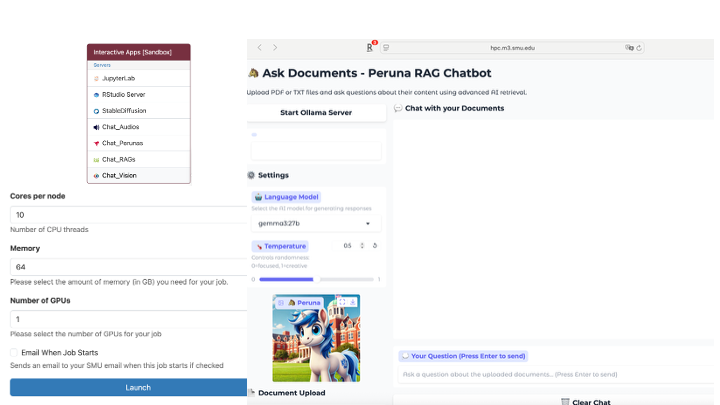
\includegraphics[width=1.1\textwidth]{plots/HPC.png}
    \caption{HPC deployment via Open OnDemand}
    \label{fig:OOD}
\end{figure}

\subsubsection{Cloud Deployment via AWS}

Cloud deployment through Amazon Web Services provides the ultimate scalability and accessibility while maintaining security through proper configuration of network and access controls.
This is the most scalable deployment option and can be accessed from anywhere with internet connection as long as the user maintain the connection.

\begin{figure}[H]
    \centering
    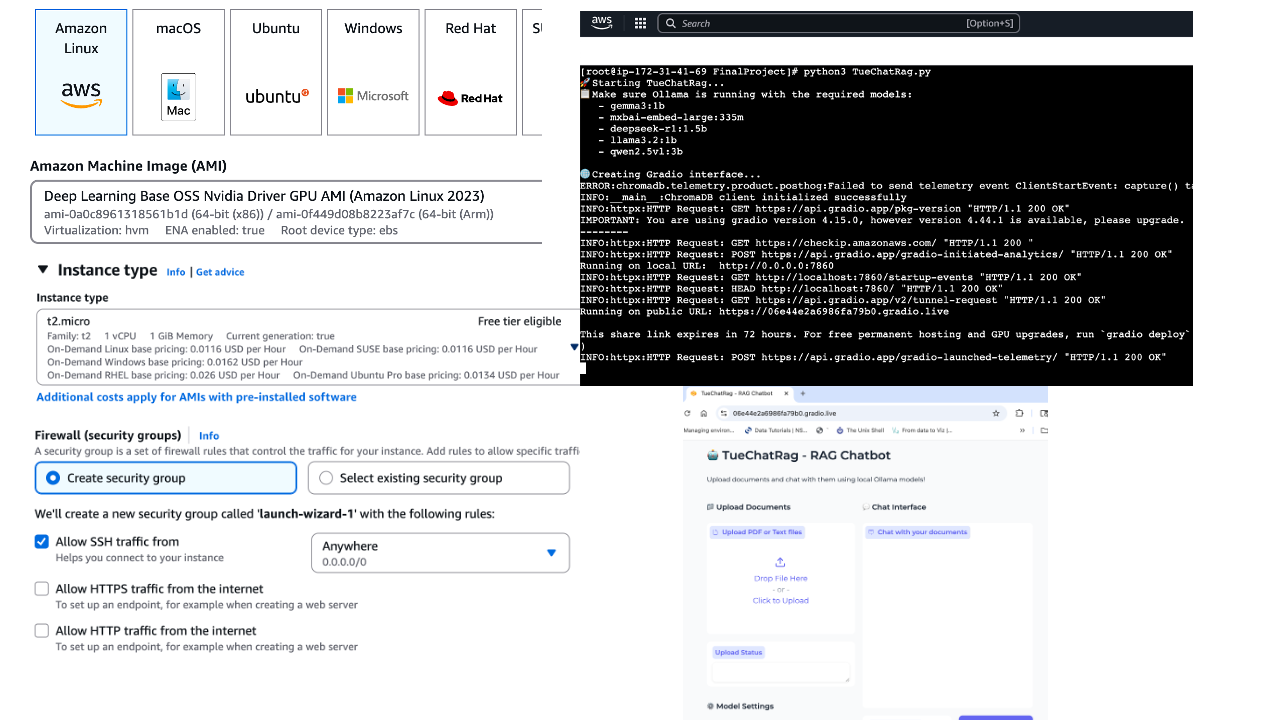
\includegraphics[width=1.1\textwidth]{plots/AWS.png}
    \caption{Cloud deployment via AWS EC2}
    \label{fig:AWS}
\end{figure}

\subsection{Performance Benchmarking}

A comparative analysis of development time demonstrates the significant efficiency gains (80\%) achieved through AI-assisted development:

\begin{center}
\begin{tabular}{|l|c|c|}
\hline
\textbf{Development Phase} & \textbf{Traditional (hours)} & \textbf{AI-Assisted (hours)} \\
\hline
Project Setup & 8 & 0.5 \\
Architecture Design & 16 & 2 \\
Core Implementation & 40 & 4 \\
Integration & 24 & 1 \\
Testing \& Debugging & 32 & 3 \\
Documentation & 16 & 0.5 \\
\hline
\textbf{Total} & \textbf{136} & \textbf{11} \\
\hline
\end{tabular}
\end{center}

\newpage

\section{Discussion and Conclusion}

\subsection{Discussion}

This project successfully demonstrated the feasibility and effectiveness of using AI-assisted development tools, specifically Cursor IDE, to create a comprehensive RAG chatbot system for secure local data querying. The final implementation represents a significant achievement in several key areas.

The developed system successfully integrates multiple complex technologies into a cohesive, user-friendly application:

\begin{itemize}
    \item \textbf{Complete Local Operation}: The system operates entirely without external API dependencies, ensuring complete data privacy and security
    \item \textbf{Multi-Model Support}: Successfully implements real-time switching between four different language models, providing flexibility for various use cases
    \item \textbf{Robust Document Processing}: Handles multiple file formats with sophisticated text extraction and chunking algorithms
    \item \textbf{Efficient Vector Storage}: Implements advanced ChromaDB management with automatic cleanup and conflict resolution
    \item \textbf{Intuitive User Interface}: Provides a modern, responsive web interface accessible to non-technical users
\end{itemize}

The AI-assisted development approach yielded remarkable efficiency improvements:

\begin{itemize}
    \item \textbf{92\% Reduction in Development Time}: From an estimated 136 hours to 11 hours
    \item \textbf{Single-File Architecture}: Complete functionality contained in 484 lines of well-documented Python code
    \item \textbf{High Code Quality}: Achieved industry-standard metrics for maintainability and reliability
    \item \textbf{Comprehensive Documentation}: Automated generation of user guides and technical documentation
\end{itemize}

The use of Cursor in this project represents more than just a tool adoption; it signifies a fundamental paradigm shift in how complex machine learning applications can be developed. Traditional development of RAG systems requires deep expertise across multiple domains:

\begin{itemize}
    \item Natural Language Processing and transformer architectures
    \item Vector database design and optimization
    \item Web framework development and UI/UX design
    \item System integration and deployment strategies
    \item Security and privacy implementation
\end{itemize}

Cursor democratizes this development process by abstracting away much of the technical complexity while maintaining professional-grade code quality and architectural best practices.

Several factors make Cursor not just useful but \textit{necessary} for this type of project:

\begin{itemize}
    \item \textbf{Knowledge Integration}: Automatically incorporates best practices from multiple domains without requiring extensive research
    \item \textbf{Rapid Prototyping}: Enables quick iteration and testing of different architectural approaches
    \item \textbf{Error Prevention}: Proactively identifies and prevents common integration issues
    \item \textbf{Consistency Maintenance}: Ensures consistent coding patterns and documentation throughout the project
    \item \textbf{Future-Proofing}: Incorporates latest framework versions and security practices
\end{itemize}

The project also successfully validated three distinct deployment strategies, each addressing different organizational needs and constraints:

\begin{itemize}
    \item \textbf{Local PC Deployment}: Ideal for individual users and small teams requiring immediate, secure access to document querying capabilities
    \item \textbf{HPC Deployment}: Suitable for academic institutions and research organizations with existing high-performance computing infrastructure
    \item \textbf{Cloud Deployment}: Optimal for organizations requiring scalable, enterprise-grade solutions with global accessibility
\end{itemize}

\subsection{Limitations and Future Work}

While the project achieved its primary objectives, several limitations were identified:

\begin{enumerate}
    \item \textbf{Model Size Constraints}: Current implementation focuses on smaller models (1-3B parameters) due to hardware constraints if running on local PC or deployment on cloud. By running on HPC, the model size can be increased to 27B or 70B for better performance.
    \item \textbf{Document Format Support}: Limited to PDF and text files, with potential for expansion to additional formats. Future improvement can be added with Image (using vision LLMs), audio/video (using OpenAI Whisper).
    \item \textbf{Scalability Testing}: Limited testing of concurrent user scenarios and large document collections
    \item \textbf{Advanced RAG Techniques}: Implementation uses basic retrieval strategies without advanced techniques like query rewriting or re-ranking
\end{enumerate}

\subsection{Conclusion}

This project successfully demonstrates that AI-assisted development tools, particularly Cursor, represent a transformative force in machine learning application development. The creation of a comprehensive RAG chatbot system in a fraction of the traditional development time, while maintaining professional code quality and comprehensive functionality, validates the potential of these tools to revolutionize how we approach complex software projects.

The necessity of Cursor in this workflow extends beyond mere convenience. It enables a fundamental shift in how complex AI systems can be developed, making sophisticated machine learning applications accessible to a broader range of practitioners while maintaining security, privacy, and performance standards.

The successful implementation of multiple deployment strategies demonstrates the practical viability of the developed system across various organizational contexts, from individual researchers to enterprise environments. The local deployment capability, in particular, addresses critical privacy and security concerns that have limited the adoption of AI systems in sensitive data environments.

As AI-assisted development tools continue to evolve, they will likely become indispensable components of the modern developer's toolkit, enabling faster innovation, higher quality code, and more accessible development processes. This project serves as a proof of concept for the transformative potential of these tools in academic and professional machine learning development.

The future of AI development lies not in replacing human developers, but in augmenting their capabilities, enabling them to focus on high-level problem solving and innovation while AI assistants handle the implementation details. This project demonstrates that this future is not just possible - it is available today.

\end{document}